\documentclass{article}
\usepackage{tikz}
\usepackage{pgfplots}
\usepackage{svg}
\usepackage{amsmath}
\usepackage{array}
\usepackage[skins]{tcolorbox}
\usepackage[version=4]{mhchem}
\usepackage[a4paper, total={6in, 9in}]{geometry}
\usepackage{fourier}
\usepackage{xymtex}
\usepackage{textcomp}
\usepackage{eurosym}
\usepackage{caption}
\usepackage{longtable}
\usepackage{float}
\usepackage{attachfile}
\usepackage{multirow}
\usepackage{amsfonts} 
\usepackage{tabularray}
\usepackage{colortbl}
\usepackage{xcolor}
\usepackage{graphicx}
\usepackage[table]{xcolor}
\UseTblrLibrary{booktabs}
\usepackage[bottom]{footmisc}

\captionsetup[table]{name=Tabella}
%<\pagenumbering{gobble}
\setcounter{secnumdepth}{2}


\renewcommand*\contentsname{Indice}
\setcounter{tocdepth}{3}
\setcounter{secnumdepth}{2}
\pgfplotsset{compat=1.15}


\title{Relazione di laboratorio - Periodo di un pendolo semplice}
\author{Federico Cesari}
\date{Aprile 2024}





%%%%%%%%%%%%%%%%%%%%%%%%%%%%%%%%%%%%%%%%%%%%%%%%%%%%%%%%%
%%				INIZIO DOC
%%%%%%%%%%%%%%%%%%%%%%%%%%%%%%%%%%%%%%%%%%%%%%%%%%%%%%%%%


\begin{document}
\begin{titlepage}
	\begin{center}
		\vspace*{1cm}
		
		\textbf{\LARGE Relazione di laboratorio - Pendolo semplice}
		
		\vspace{0.3cm}
		\large \textit{Misura del periodo di un pendolo semplice} \\
		
		\vspace{0.5cm}
		\Large Federico Cesari \\
		
		\small 1096759 
		\vspace{0.2cm}
		
		\small Gruppo 5
		
		
		\vspace{3cm}
		\begin{center}
			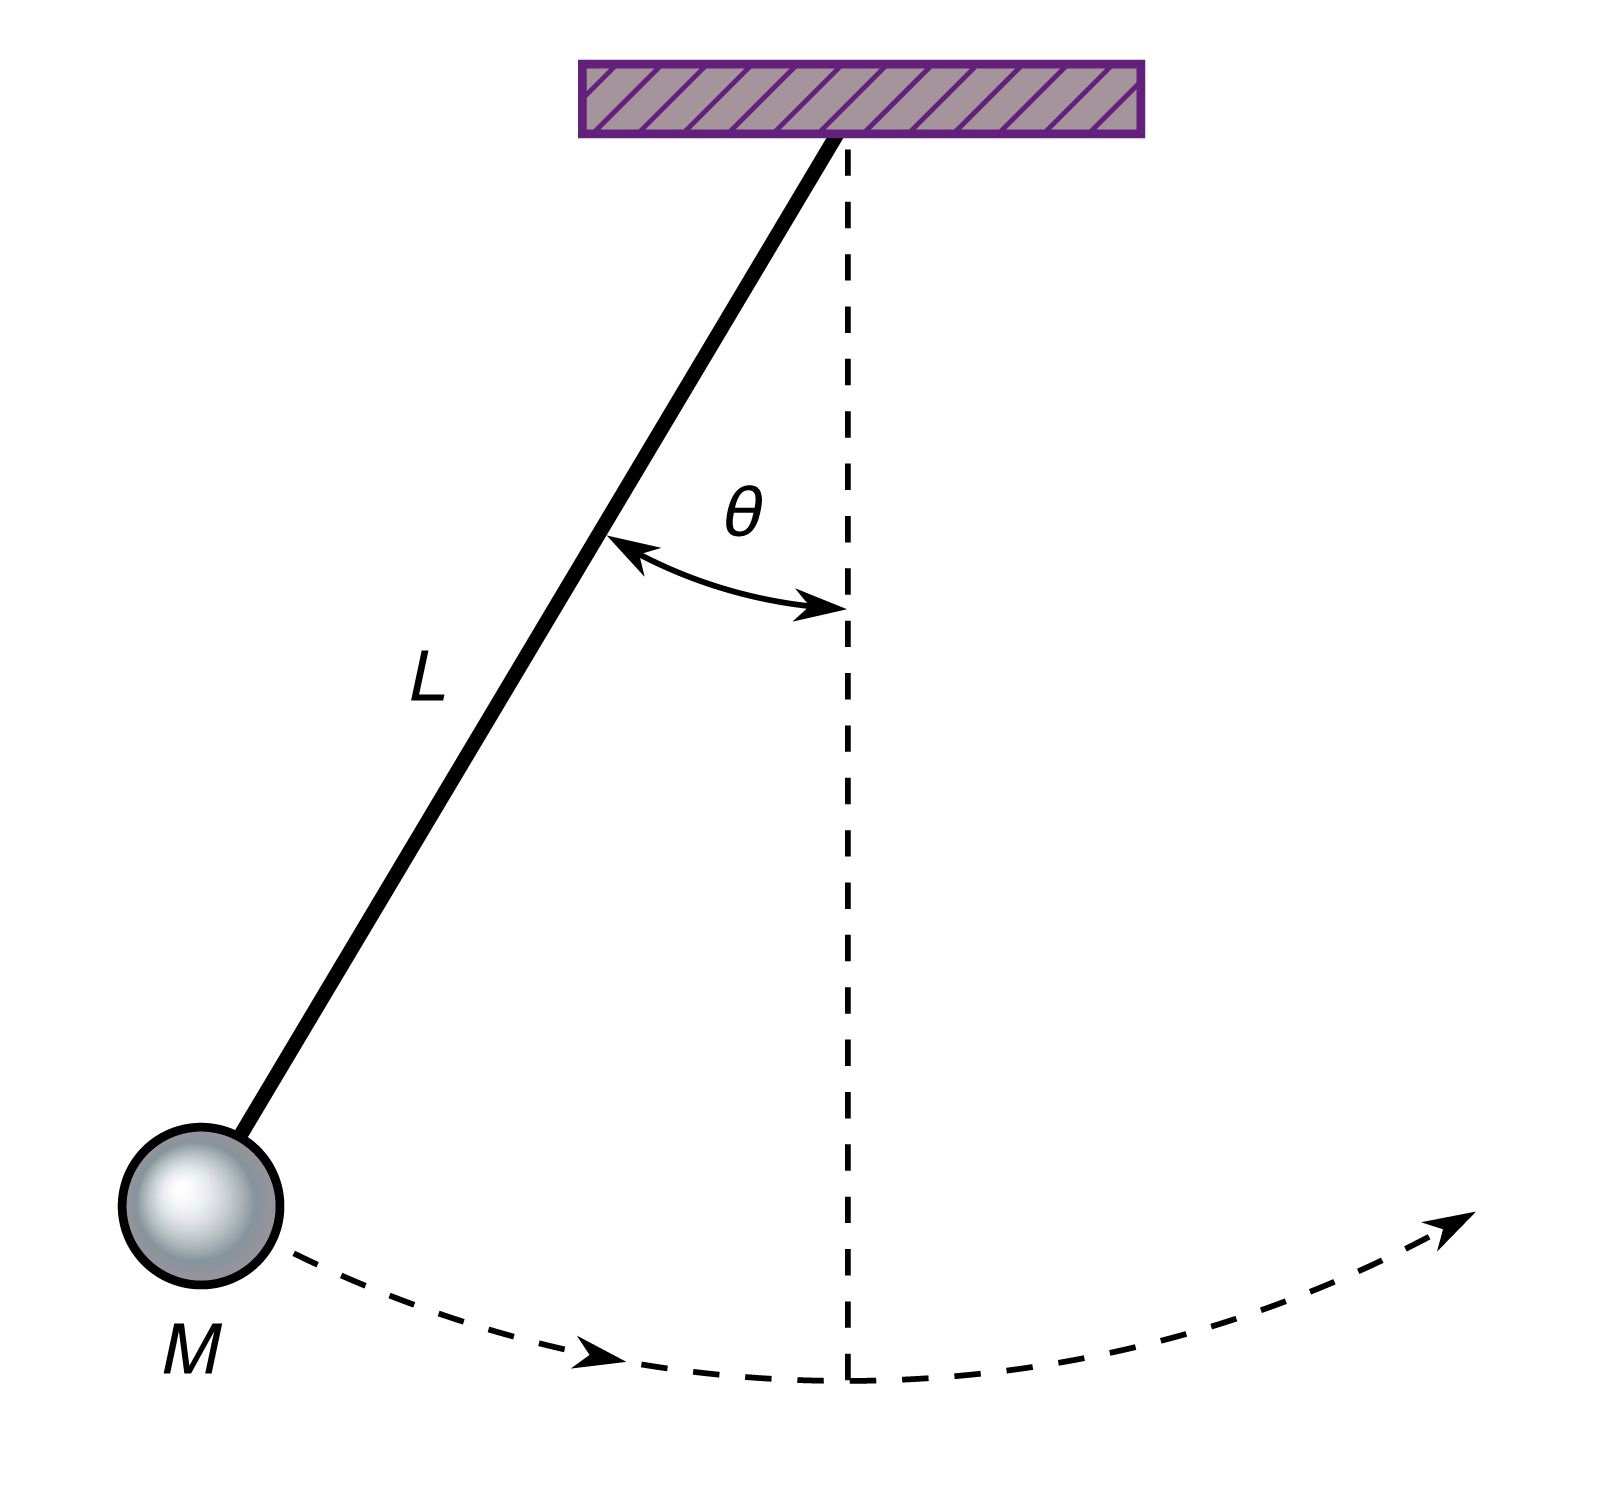
\includegraphics[scale=0.1]{IMG_0200.jpeg}	
		\end{center}
		
		
		
		\vfill
		
		
		
		corso A\\
		Università degli studi di Torino, Torino\\
		4 aprile 2024\\
		
		
	\end{center}
\end{titlepage}
\tableofcontents

\newpage
\section{Scopo dell’esperienza}
L'esperienza di laboratorio ha lo scopo di studiare il periodo di un pendolo semplice del quale conosciamo le espressioni del periodo teorico (in condizioni ideali e prive di attrito) al variare della sua lunghezza e dell'angolo di partenza. Verrà quindi misurato il periodo e se ne osserverà la variazione in funzione dell'angolo, della lunghezza e della massa appesa ad esso.

\section{Premesse teoriche}
\textcolor{red}{aggiungi equazioni}

\section{Strumentazione}
\begin{table}[H]
	\centering
	\begin{tabular}{@{}ll@{}}
		\textbf{Strumento} & \textbf{Sensibilità} \\ \midrule
		Cr. Analogico      & $0.2$s               \\
		Cr. Digitale       & $0.01$s              \\
		Fotocellula        & $0.001$s             \\
		Goniometro         & $1^\circ$            \\
		Asta graduata      & $0.1$cm              \\
		Calibro            & $0.01$mm             \\
		Bilancia digitale  & $1$g                 \\ \bottomrule
	\end{tabular}
\end{table}





%%%%%%%%%%%%%%%%%%%%%%%%%%%%%%%%%%%%%%%%%%%%%%%%%%%%%%%%%
%%				SCELTA STRUMENTO
%%%%%%%%%%%%%%%%%%%%%%%%%%%%%%%%%%%%%%%%%%%%%%%%%%%%%%%%%




\section{Scelta strumento di misura}

Al fine di stabilire il migliore strumento di misura per le succesive misurazioni, registro 8 misure del periodo del pendolo prima con un angolo di partenza $\vartheta = 5^\circ$ e poi con $\vartheta = 30^\circ$ utilizzando un cronometro analogico, uno digitale e una fotocellula. Lo strumento che mostrerà discrepanze significative tra il periodo calcolato con $\vartheta = 5^\circ$ e $\vartheta = 30^\circ$ sarà quello utilizzato per i testi successivi. Procedo quindi con le misurazioni dei periodi del pendolo a cui è stata agganciata una sfera di massa $m = (110 \pm 1)g$

\textcolor{red}{sistema valori per C.Analogico.}

\vspace{1cm}
\begin{minipage}{0.5\textwidth}
\begin{table}[H]
	\hspace{-1.3cm}
	\begin{tabular}{@{}lrrr@{}}
		&\textbf{C.Analogico} & \textbf{C. Digitale} & \textbf{Fotocellula} \\ \cmidrule(l){2-4} &\multicolumn{1}{l}{$T(s) \pm 0.2s$} & \multicolumn{1}{l}{$T(s) \pm 0.01s$}   & \multicolumn{1}{l}{$T(s) \pm 0.001s$}    \\ \cmidrule(l){2-4} 
		
		\multicolumn{1}{c}{}  
		& 1.6   & 1.63   & 1.702     \\
		\colorbox{orange!40}{$\vartheta = 5^\circ$}   & 1.7   & 1.65   & 1.703     \\
		& 1.5   & 1.60   & 1.703     \\ 
		& 1.7   & 1.71   & 1.703     \\
		& 1.7   & 1.71   & 1.703     \\
		& 1.7   & 1.65   & 1.702     \\
		& 1.6   & 1.70   & 1.703     \\
		& 1.7   & 1.70   & 1.703     \\ \arrayrulecolor{black!100}\specialrule{1.2pt}{0.5\jot}{0.5pc}
		
		$\mathbf{\bar{T}_{5}(s)}$ & \textbf{1.65}    & \textbf{1.67}  & \textbf{1.703}  \\
		$\sigma_{T_{5}}$   & 0.05    & 0.02  & 0.000 \\                          
	\end{tabular}
\end{table}
\end{minipage}
\begin{minipage}{0.5\textwidth}
\begin{table}[H]
	\centering
	\begin{tabular}{@{}lrrr@{}}
		&\textbf{C.Analogico} & \textbf{C. Digitale} & \textbf{Fotocellula} \\ \cmidrule(l){2-4} &\multicolumn{1}{l}{$T(s) \pm 0.2s$} & \multicolumn{1}{l}{$T(s) \pm 0.01s$}   & \multicolumn{1}{l}{$T(s) \pm 0.001s$}    \\ \cmidrule(l){2-4} 
		
		\multicolumn{1}{c}{}  
													& 1.8   & 1.65   & 1.733     \\
		\colorbox{blue!40}{$\vartheta = 30^\circ$}  & 1.7   & 1.67   & 1.733     \\
													& 1.6   & 1.70   & 1.733     \\ 
													& 1.7   & 1.62   & 1.733     \\
													
													& 1.7   & 1.70   & 1.731     \\
													& 1.8   & 1.72   & 1.733     \\
													& 1.7   & 1.80   & 1.733     \\
													& 1.6   & 1.69   & 1.732     \\ \arrayrulecolor{black!100}\specialrule{1.2pt}{0.5\jot}{0.5pc}

		$\mathbf{\bar{T}_{30}(s)}$ & \textbf{1.70}    & \textbf{1.69}  & \textbf{1.715}  \\
		$\sigma_ {T_{30}}$   & 0.08    & 0.03  & 0.0005 \\                          
	\end{tabular}
\end{table}
\end{minipage}
\vspace{1cm}

\noindent
Da questi primi set di dati noto subito che la deviazione standard dei periodi misurati dal cronometro digitale è più grande della sensibilità dello strumento, quindi dovrei scegliere la deviazione standard come errore sulla singola misura.


Invece per evidenziare quale dei tre strumenti fornisca periodi significativamente differenti per i due angoli di partenza sottopongo le coppie di periodi medi a un test Z:


\begin{table}[H]
	\centering
	\begin{tabular}{@{}lrr@{}}
		\toprule
		\multicolumn{1}{c}{Z} & \multicolumn{1}{l}{$\sigma_{\bar{T}_5}$} & \multicolumn{1}{l}{$\sigma_{\bar{T}_{30}}$} \\ \midrule
		$z_{\text{an.}}$      & \textit{\textbf{0.234}}                  & \textit{\textbf{0.234}}                   \\
		$z_{\text{dig.}}$     & \textit{\textbf{0.170}}                  & \textit{\textbf{0.132}}                   \\
		$z_{\text{fot.}}$     & \textit{\textbf{22.8}}                   & \textit{\textbf{14.2}}                    \\ \bottomrule
	\end{tabular}
\end{table}

Il test mostra che i periodi misurati con i cronometri analogico e digitale con ancgoli di partenza $\vartheta = 5^\circ$ e $\vartheta = 30^\circ$, risultano essere compatibili con livelli di significatività \textcolor{red}{maggiori dell'80\% (specifica bene i valori)}. Per quanto riguarda i periodi registrati con la fotocellula questi risultano \textcolor{red}{appartenere a popolazioni differenti} e posso quindi affermare che lo strumento che fornisce periodi significativamente differenti per i due angoli di partenza sia proprio la fotocellula.








%%%%%%%%%%%%%%%%%%%%%%%%%%%%%%%%%%%%%%%%%%%%%%%%%%%%%%%%%
%%				DIPENDENZA THETA   00000
%%%%%%%%%%%%%%%%%%%%%%%%%%%%%%%%%%%%%%%%%%%%%%%%%%%%%%%%%

\newpage
\section{Dipendenza dall’angolo}
La prima parte dell'esperienza consiste nel verificare la dipendenza di $T$, periodo del pendolo a cui è stata attaccata una sferetta di legno di massa $m = (10 \pm 1)g$, da $\vartheta$, angolo di partenza.  Per prima cosa si procede alla misurazoine della lunghezza del pendolo. Attraverso l'asta graduata misuro prima la distanza da terra alla cima del pendolo ($L_C$) e poi la distanza da terra al centro della sfera appesa ($L_F$)\footnote{Avrei potuto misurare il diametro della sfera con il calibro e aggiungere il raggio della sfera successivamente invece che includerlo nelle misura di cima e fondo, tuttavia la sensibilità dell'asta e il fatto che questa non fosse perfettamente perpendicolare ha reso gli errori di $L_C$ e $L_F$ troppo grossolani rendendo così inutile la maggiore cura nella misura del raggio.}. 

\begin{table}[H]
	\centering
	\begin{tabular}{@{}cc@{}}
		\textbf{Cima} & \textbf{Fondo}\\ \midrule
		$L_C(\text{cm}) \pm 0.1\text{cm}$  & $L_F(\text{cm}) \pm 0.1\text{cm}$ \\ \midrule
		89.0 & 16.8  \\ \bottomrule
	\end{tabular}
\end{table}

Ricavo quindi la lunghezza del pendolo:

\[
l = L_C + L_F = (72.2 \pm 0.2) \text{cm}. \footnote{Propago l'errore linearmente ($\left(0.1 + 0.1 \right)\text{cm} = 0.2\text{cm}$) perché essendo solo due misure (per di più effettuate con un asta graduata imperfetta) rischio di sottostimare l'errore sommandolo in quadratura}
\] 


A questo punto prendo tre misurazioni del periodo del pendolo,  partendo da un angolo di partenza di $5^\circ$. Continuo a prendere le misure avanzando di $5^\circ$ fino ad arrivare a $30^\circ$.	



\begin{table}[H]
	\centering
	\begin{tabular}{@{}lrrrrrr@{}}
		& $\mathbf{5^\circ}$ & $\mathbf{10^\circ}$ & $\mathbf{15^\circ}$ & $\mathbf{20^\circ}$ & $\mathbf{25^\circ}$ & $\mathbf{30^\circ}$  \\ \cmidrule(l){2-7}   
		& $T(s) \pm 0.001s$ & $T(s) \pm 0.001s$   & $T(s) \pm 0.001s$ & $T(s) \pm 0.001s$ & $T(s) \pm 0.001s$ & $T(s) \pm 0.001s$  \\ \cmidrule(l){2-7} 
		
		\multicolumn{1}{c}{}  
		
		&1.703 & 1.706 & 1.710 & 1.715 & 1.723 & 1.730  \\
		&1.702 & 1.706 & 1.710 & 1.715 & 1.723 & 1.731 \\
		&1.701 & 1.706 & 1.710 & 1.715 & 1.723 & 1.731 \\
		
		\arrayrulecolor{black!100}\specialrule{1.2pt}{0.5\jot}{0.5pc}
		
		$\mathbf{\bar{T}(s)}$ & \textbf{1.702}    & \textbf{1.706}  & \textbf{1.710} & \textbf{1.715} & \textbf{1.723} &  \textbf{1.731}        
	\end{tabular}
\end{table}

\noindent
Dall'espressione del periodo del pendolo sappiamo che il periodo è direttamente proporzionale a $\sin\left(\vartheta/2\right)^2$, più precisamente:
\[
T = T_0 \left[ 1 + \frac{1}{4}\sin{\left(\vartheta/2\right)}^2 \right]
\]
Se dovessi riportare su un grafico i periodi sperimentali in funzione di $x = \sin{\left(\vartheta/2\right)}^2$ mi aspetto quindi un andamento lineare e più precisamente una retta del tipo

\[
y = T_0 + \frac{T_0}{4}x
\]

\noindent
Per verificare ciò mi avvalgo del metodo dei minimi quadrati...
\textcolor{red}{inserire qualche informazione a riguardo}

\subsubsection{Minimi quadrati}
Appurato che $T$ e $\sin{\left(\vartheta/2\right)}^2$ siano \textit{teoricamente} linearmente correlati, è di mio interesse trovare quale retta della forma $y = A + Bx$ meglio interpola i dati sperimentali così da appurare se i valori misurati soddisfano la attesa teorica che $y$ sia lineare in $x$. 

Posso fare questo avvalendomi del metodo dei minimi quadrati che ha  proprio lo scopo di determinare i parametri che legano due variabili legate da essi, nel mio caso due variabili $x$ e $y$ legati da due parametri $A$ e $B$.

\vspace{2cm}
Questo metodo necessita delle assunzioni importanti: 

\begin{enumerate}
	\item Le misure siano statisticamente indipendenti;
	\item Una delle due variabili (sceglierò la $x$) abbia errori trascurabili rispetto all'altra \footnote{Giudico un errore come trascurabile rispetto all'altro quando si trovano in rapporto 1 a 3,4,5.}.
	\item Gli errori della variabile $y$ siano distribuiti normalmente.
\end{enumerate}
\textcolor{red}{preso letteralmente dal Cannelli}

Per rispettare la seconda assunzione confronto gli errori relativi delle mie due variabili.

\begin{minipage}{0.5\textwidth}
\begin{table}[H]
	\centering
	\begin{tabular}{@{}ccc@{}}
		\multicolumn{3}{c}{$\mathbf{T}$} \\ \midrule
		$T(s)$ & $\delta_T (s)$ & $\delta_T / T$ \\ \midrule
		1.702 & 0.001 & \textbf{0.000339} \\
		1.706 & 0.001 & \textbf{0.000338} \\
		1.710 & 0.001 & \textbf{0.000337} \\
		1.715 & 0.001 & \textbf{0.000336} \\
		1.723 & 0.001 & \textbf{0.000335} \\
		1.731 & 0.001 & \textbf{0.000333}  \\ \bottomrule   
	\end{tabular}
\end{table}
\end{minipage}
\begin{minipage}{0.5\textwidth}
\begin{table}[H]
	\centering
	\begin{tabular}{@{}ccc@{}}
		
		\multicolumn{3}{c}{$y = \mathbf{sin{\left(\vartheta/2\right)}^2}$} \\ \midrule
		$y$ & $\delta_y$ & $\delta_y / y$ \\ \midrule
		0.0019&0.00075 & \textbf{0.398} \\
		0.0076&0.0015 & \textbf{0.198}  \\
		0.017&0.0023 & \textbf{0.132}  \\ 
		0.030&0.0030 & \textbf{0.099}  \\
		0.047&0.0037 & \textbf{0.078}  \\
		0.067&0.0044 & \textbf{0.065}  \\ \bottomrule  
	\end{tabular}
\end{table}
\end{minipage}
\footnote{Lascio 3 cifre significative negli errori relativi del periodo per evidenziarne le piccole discrepanze.}
\vspace{1cm}

Come si può leggere nelle tabelle l'errore associato alle misure dei periodi è perfettamente trascurabile rispetto a quello associato al seno, quindi scelgo di portare le misure del periodo sull'asse $x$ e quelle del seno sull'asse $y$. 

\noindent
Procedo al calcolo dei parametri $A$ e $B$ e dei rispettivi errori:

\[
\mathbf{A} = -3.68 \qquad \mathbf{\sigma_A} = 0.179
\]
\[
\mathbf{B} = 2.16 \qquad \mathbf{\sigma_B} = 0.105
\]

\begin{minipage}{0.3\textwidth}
\textcolor{red}{l'errore sulla x è da scrivere?}
\begin{table}[H]
	\centering
	\begin{tabular}{@{}ll@{}}
		$T(s) \pm \delta_T$ & $\sin{\left(\vartheta/2\right)}^2 \pm \delta_y$ \\ \midrule
		1.702&0.0019    \\
		1.706&0.0076    \\
		1.710&0.0170    \\
		1.715&0.0302    \\
		1.723&0.0468    \\
		1.731&0.0669    \\	\bottomrule
\end{tabular}
\end{table}
\end{minipage}
\begin{minipage}{0.7\textwidth}
\begin{figure}[H]
	\centering
	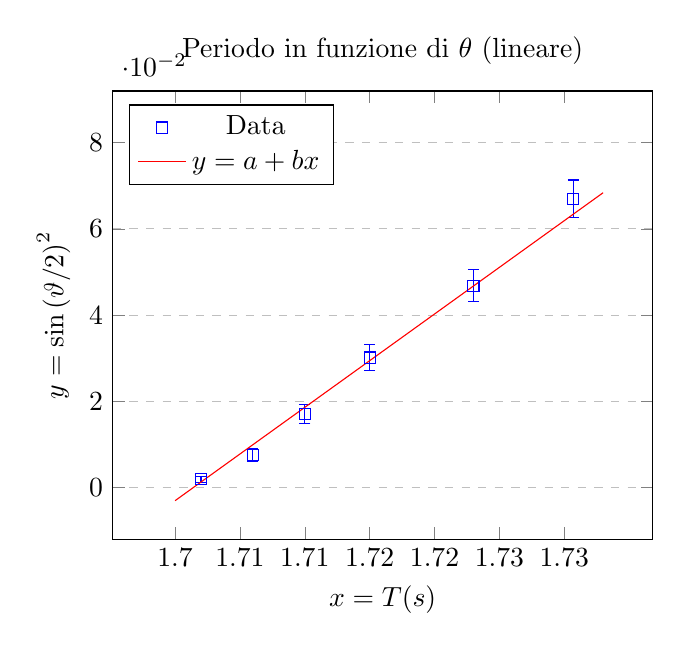
\begin{tikzpicture}
		\begin{axis}[
			title={Periodo in funzione di $\theta$ (lineare)},
			xlabel={$x = T(s)$},
			ylabel={$y = \sin{\left( \vartheta / 2\right) }^2$},
			xmin=1.7, xmax=1.732,
			ymin=0, ymax=0.08,
			xtick={1.7,1.705,1.71,1.715,1.72,1.725,1.73},
			ytick={0,0.02,0.04,0.06,0.08},
			legend pos=north west,
			ymajorgrids=true,
			grid style=dashed,
			enlargelimits=0.15,
			]
			
			\addplot[
			only marks,
			color=blue,
			mark=square,
			error bars/.cd,
			y dir=both, y explicit
			]
			coordinates {
				(1.702,0.0019027) +- (0,0.00075825)
				(1.706,0.0075961) +- (0,0.00151074)
				(1.710,0.0170371) +- (0,0.00225173)
				(1.715,0.0301537) +- (0,0.00297558)
				(1.723,0.0468461) +- (0,0.00367678)
				(1.7307,0.0669873) +- (0,0.00435)
			};
			\addplot[
				domain=1.7:1.733, 
				samples=100, 
				color=red, 
				] 
				{2.16490*x -3.68337};
			\node[] at (axis cs: 1.73,1) {absolute in pgfplots coordinates};
			\legend{Data,$y=a+bx$}
		\end{axis}
	\end{tikzpicture}
	\caption{$T\left( \sin{\left( \vartheta / 2\right) }^2\right) $}
\end{figure}
\end{minipage}

\begin{figure}[H]
	\centering
	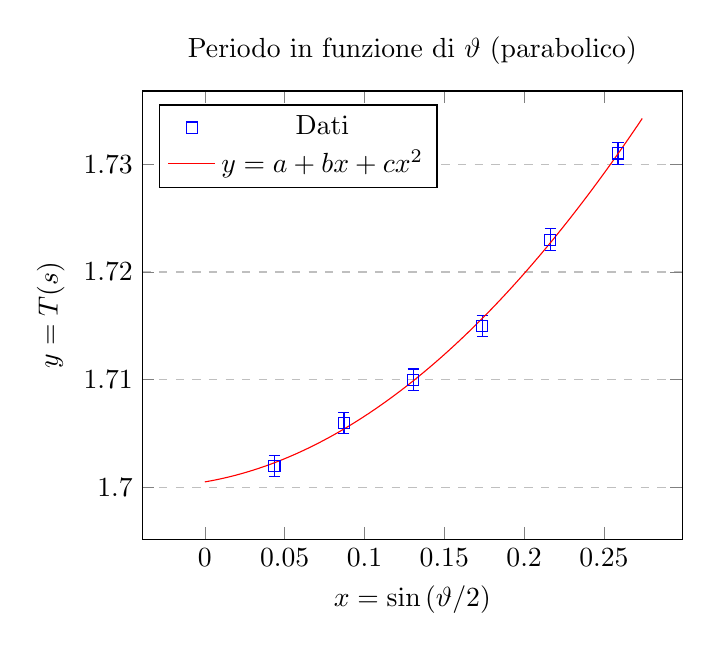
\begin{tikzpicture}
		\begin{axis}[
			title={Periodo in funzione di $\vartheta$ (parabolico)},
			ylabel={$y = T(s)$},
			xlabel={$x = \sin{\left( \vartheta / 2\right) }$},
			xmin=0, xmax=0.26,
			ymin=1.700, ymax=1.732,
			xtick={},
			ytick={},
			tick label style={/pgf/number format/fixed},
			legend pos=north west,
			ymajorgrids=true,
			grid style=dashed,
			enlargelimits=0.15,
			]
			
			\addplot[
			only marks,
			mark=square,
			color=blue,
			error bars/.cd,
			y dir=both, y explicit
			]
			coordinates {
				(0.0436194,1.702) +- (0,0.001)
				(0.0871557,1.706) +- (0,0.001)
				(0.1305262,1.710) +- (0,0.001)
				(0.1736482,1.715) +- (0,0.001)
				(0.2164396,1.723) +- (0,0.001)
				(0.2588190,1.731) +- (0,0.001)
			};
			\addplot[
			domain=0:0.274, 
			samples=100, 
			color=red, 
			] 
			{0.35725602*x^2 + 0.0252062*x + 1.700522};
			\legend{Dati,$y=a+bx+cx^2$}
		\end{axis}
	\end{tikzpicture}
	\caption{Rappresentazione grafica dei dati sperimentali con errori ridotti.}
\end{figure}


Calcolo il valore di g:
\[
T_0 = 2\pi\sqrt{\frac{l}{g}} \qquad \to \qquad T_0^2 = 4\pi^2\frac{l}{g}
\] 
\[
g = \frac{4l\pi^2}{T_0^2}
\]

poiché sappiamo che

\[
T = T_0 + \frac{T_0}{4}y \qquad \to \qquad y = 4\frac{T-T_0}{T_0} \qquad \to \qquad y = 4\frac{T}{T_0} - 4
\]
\[
b = \frac{4}{T_0} \qquad \to \qquad T_0 = \frac{4}{b}
\]

Quindi

\[
\mathbf{g = \frac{l\pi^2}{4}b^2}
\]

Calcolo l'errore associato a g:
\[
\sigma_g = \sqrt{\left(\frac{\partial g}{\partial l} \right)^2\sigma_l^2 + \left(\frac{\partial g}{\partial b} \right)^2 \sigma_b^2}
\]
\[
\sigma_g = 	\sqrt{\left(\frac{b^2\pi^2}{4}\right)^2 \sigma_l^2 + \left( \frac{lb\pi^2}{2}  \right)^2 \sigma_b^2	 }
\]

\subsubsection{Test Z per g}

Ottengo $g = ...$ ... Scelgo livello di significatività = 0.05.






%%%%%%%%%%%%%%%%%%%%%%%%%%%%%%%%%%%%%%%%%%%%%%%%%%%%%%%%%
%%				DIPENDENZA ELLE     LLLLL
%%%%%%%%%%%%%%%%%%%%%%%%%%%%%%%%%%%%%%%%%%%%%%%%%%%%%%%%%

\newpage
\section{Dipendenza dalla lunghezza}

\begin{figure}[H]
	\centering
	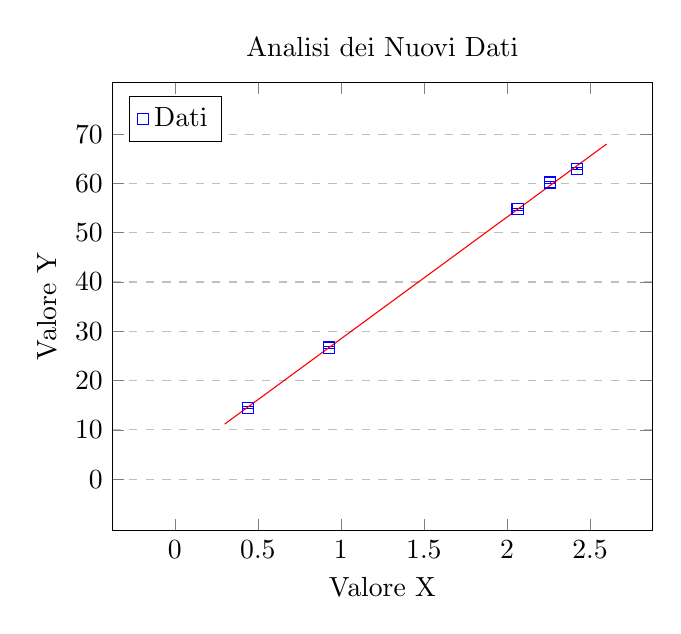
\begin{tikzpicture}
		\begin{axis}[
			title={Analisi dei Nuovi Dati},
			xlabel={Valore X},
			ylabel={Valore Y},
			xmin=0, xmax=2.5,
			ymin=0, ymax=70,
			xtick={0,0.5,1,1.5,2,2.5},
			ytick={0,10,20,30,40,50,60,70},
			legend pos=north west,
			ymajorgrids=true,
			grid style=dashed,
			enlargelimits=0.15,
			]
			
			\addplot[
			only marks,
			color=blue,
			mark=square,
			error bars/.cd,
			y dir=both, y explicit
			]
			coordinates {
				(2.260011111,60.20) +- (0,0.2)
				(0.9267271111,26.70) +- (0,0.2)
				(0.4391271111,14.50) +- (0,0.2)
				(2.422173444,63.00) +- (0,0.2)
				(2.064011111,54.80) +- (0,0.2)
			};
			\addplot[
			domain=0.3:2.6, 
			samples=100, 
			color=red, 
			] 
			{ 24.7131*x + 3.74511};
			\legend{Dati}
		\end{axis}
	\end{tikzpicture}
	\caption{Rappresentazione grafica dei dati sperimentali con errori.}
\end{figure}


\subsection{Confronto parametri retta}





%%%%%%%%%%%%%%%%%%%%%%%%%%%%%%%%%%%%%%%%%%%%%%%%%%%%%%%%%
%%				DIPENDENZA MASSA     MMMM
%%%%%%%%%%%%%%%%%%%%%%%%%%%%%%%%%%%%%%%%%%%%%%%%%%%%%%%%%

\newpage
\section{Dipendenza dalla massa}








%%%%%%%%%%%%%%%%%%%%%%%%%%%%%%%%%%%%%%%%%%%%%%%%%%%%%%%%%
%%				    CONCLUSIONI
%%%%%%%%%%%%%%%%%%%%%%%%%%%%%%%%%%%%%%%%%%%%%%%%%%%%%%%%%

\newpage
\section{Conclusioni}



\end{document}
